\documentclass{beamer}
\mode<presentation>
\usepackage{amsmath}
\usepackage{amssymb}
\usepackage{adjustbox}
\usepackage{subcaption}
\usepackage{enumitem}
\usepackage{multicol}
\usepackage{mathtools}
\usepackage{listings}
\usepackage{url}
\def\UrlBreaks{\do\/\do-}
\usetheme{AnnArbor}
\usecolortheme{spruce}
\setbeamertemplate{footline}
{
  \leavevmode%
  \hbox{%
  \begin{beamercolorbox}[wd=\paperwidth,ht=2.25ex,dp=1ex,right]{author in head/foot}%
    \insertframenumber{} / \inserttotalframenumber\hspace*{2ex} 
  \end{beamercolorbox}}%
  \vskip0pt%
}
\setbeamertemplate{navigation symbols}{}

\providecommand{\nCr}[2]{\,^{#1}C_{#2}} % nCr
\providecommand{\nPr}[2]{\,^{#1}P_{#2}} % nPr
\providecommand{\mbf}{\mathbf}
\providecommand{\pr}[1]{\ensuremath{\Pr\left(#1\right)}}
\providecommand{\qfunc}[1]{\ensuremath{Q\left(#1\right)}}
\providecommand{\sbrak}[1]{\ensuremath{{}\left[#1\right]}}
\providecommand{\lsbrak}[1]{\ensuremath{{}\left[#1\right.}}
\providecommand{\rsbrak}[1]{\ensuremath{{}\left.#1\right]}}
\providecommand{\brak}[1]{\ensuremath{\left(#1\right)}}
\providecommand{\lbrak}[1]{\ensuremath{\left(#1\right.}}
\providecommand{\rbrak}[1]{\ensuremath{\left.#1\right)}}
\providecommand{\cbrak}[1]{\ensuremath{\left\{#1\right\}}}
\providecommand{\lcbrak}[1]{\ensuremath{\left\{#1\right.}}
\providecommand{\rcbrak}[1]{\ensuremath{\left.#1\right\}}}
\theoremstyle{remark}
\newtheorem{rem}{Remark}
\newcommand{\sgn}{\mathop{\mathrm{sgn}}}
\providecommand{\abs}[1]{\left\vert#1\right\vert}
\providecommand{\res}[1]{\Res\displaylimits_{#1}} 
\providecommand{\norm}[1]{\lVert#1\rVert}
\providecommand{\mtx}[1]{\mathbf{#1}}
\providecommand{\mean}[1]{E\left[ #1 \right]}
\providecommand{\fourier}{\overset{\mathcal{F}}{ \rightleftharpoons}}
\providecommand{\system}{\overset{\mathcal{H}}{ \longleftrightarrow}}
\providecommand{\dec}[2]{\ensuremath{\overset{#1}{\underset{#2}{\gtrless}}}}
\newcommand{\myvec}[1]{\ensuremath{\begin{pmatrix}#1\end{pmatrix}}}
\let\vec\mathbf

\lstset{
frame=single, 
breaklines=true,
columns=fullflexible
}

\numberwithin{equation}{section}

% Title Page and Document Content
\title{Solution of a differential Equation}
\author{Patnam Shariq Faraz Muhammed \\ EE24BTECH11049}
\date{} 
\begin{document}

\begin{frame}{Frame Title}
    \titlepage
\end{frame}

\begin{frame}{Question}
    \textbf{Question}:\\
    In a bank, the principal continuously increases at a rate of $r\%$ per year. Find the value of $r$ if Rs 100 doubles in 10 years \brak{\log_e2 = 0.6931}.
\end{frame}

\begin{frame}{Table}
    \textbf{Solution: }\\
    \begin{table}[ht!]
        \centering
        \begin{tabular}{|c|c|}
    \hline
    \textbf{Variable} & \textbf{Description}\\
    \hline
    $P_0$ & initial principal amount\\
    \hline
    $r$ & rate of increase per year\\
    \hline
    $t$ & time in years\\
    \hline 
    $C \& C_1$ & arbitrary constants\\
    \hline
    $P$ & principal at any time $t$\\
    \hline
\end{tabular}

        \caption{Variables used}
        \label{tab:my_label}
    \end{table}
\end{frame}

\begin{frame}{Solution}

    $P$ is the principal at any time, according to the given question, the rate of change of principal can be written as follows.

    \begin{align}
        \frac{dP}{dt} &= \brak{\frac{r}{100}} \times P \label{1}
    \end{align}

    Separation of the variables in the equation \eqref{1}
    \begin{align}
         \frac{dP}{p} &= \brak{\frac{r}{100}} \times dt \label{2}
    \end{align}
\end{frame}
\begin{frame}{Solution}
    Integration on both sides \eqref{2}
    \begin{align}
        \int{\frac{dP}{p}} &= \int{\brak{\frac{r}{100}} dt}\\
        \log_e{P} &= \frac{rt}{100} + C\\
        P &= e^{\frac{rt}{100} + C}\\
        P &= e^{\frac{rt}{100}}e^C\\
        P &= C_1e^{\frac{rt}{100}} \label{3}
    \end{align}

    At time $t = 0$, it is given that the principal is $100$, that is, $P_0 = 100$. \\ 
    Substitute in equation \eqref{3}
    \begin{align}
        100 = C_1
    \end{align}
\end{frame}
\begin{frame}{Solution}
    Principal can be written as
    \begin{align}
        P &= 100 \times e^{\frac{rt}{100}} \label{4}
    \end{align}

    At $t = 10$, the principal doubles, that is, $P = 200$, using equation \eqref{4}
    \begin{align}
        200 &= 100 \times e^{\frac{r}{10}}\\
        2 &= e^{\frac{r}{10}}\\
        \log_e{2} &= \frac{r}{10}\\
        r &= 10 \times \log_e{2}\\
        r &= 6.931
    \end{align}
\end{frame}
\begin{frame}{Differential Equation}
    The differential equation 
    \begin{align}
        \frac{dP}{dt} &= 0.06931 \times P \label{diffeq}
    \end{align}
\end{frame}

\begin{frame}{Verification of the solution computationally}
    \textbf{Euler's Method:}

    From the definition of $\frac{dy}{dx}$,
    \begin{align}
        \frac{dy}{dx} &\approx \frac{y\brak{x + h} - y\brak{x}}{h}\\
        \frac{dy}{dx} &= \frac{y_{n+1} - y_n}{h}
    \end{align}

    As per the question
    \begin{align}
        \frac{dP}{dt} &= \frac{P_{n+1} - P_n}{h}
    \end{align}

    substitute \eqref{diffeq}
    \begin{align}
        \frac{P_{n+1} - P_n}{h} &= 0.06931\times P_n
    \end{align}
\end{frame}
\begin{frame}{Difference Equations}
    We represent the the differential equation in the following difference equations:
    \begin{align}
        t_{n+1} &= t_{n}+h \\
        P_{n+1} - P_n &= 0.06931\times P_n \times h\\
        P_{n+1} &= P_{n}+h \times 0.06931 \times P_n
    \end{align}
    Where h is step and is small.
\end{frame}

\begin{frame}{Laplace transforms}
    \begin{itemize}
    \item\textbf{Laplacian Operator:}\\
         If $f\brak{t}$ is a function, the Laplace transform of that function is
        \begin{align}
            \mathcal{L}\brak{f\brak{t}} = \int_0^{\infty}{e^{-st}f\brak{t}}dt \label{lap}
        \end{align}
        \item It is linear transformation, since integral is a linear operator 
        \end{itemize}
\end{frame}
\begin{frame}{Laplace tranforms of some functions:}
\begin{itemize}
        \item \textbf{Laplace tranforms of some functions:}
        \begin{align}
            f\brak{t} &= 0 \implies F(s) = 0 \\
        f\brak{t} &= 1 \implies F(s) = \frac{1}{s} \text{ for } Re(s) > 0\\
        f\brak{t} &= t^n \implies F(s) = \frac{\Gamma\brak{a+1}}{s^{n+1}} \text{ for } Re(s) > 0 \\
        f\brak{t} &= e^{at} \implies F(s) = \frac{1}{s-a} \text{ for } Re(s) > a \\
        f\brak{t} &= \sin{at} \implies F(s) = \frac{a}{s^2 + a^2} \text{ for } Re(s) > 0 \\
        f\brak{t} &= \cos{at} \implies F(s) = \frac{s}{s^2 + a^2} \text{ for } Re(s) > 0
        \end{align}
    \end{itemize}
\end{frame}

\begin{frame}{Laplace transforms of derivatives}
    \begin{itemize}
        \item \textbf{Laplace transforms of derivatives:}
        \begin{align}
			\mathcal{L} \brak{f^{\prime}} &= s F(s) - f(0) \label{dif1} \\
			\mathcal{L} \brak{f^{\prime \prime}} &= s^2 F(s) - s f(0) - f^{\prime}(0) \label{dif2}
        \end{align}
\end{itemize}
\end{frame}
\begin{frame}{\textbf{Laplace transform of unit step function $u(t)$ :}}
		\begin{align}
			u(t) &= 
			\begin{cases} 
				1 & t \geq 0 \\
				0 & t < 0
			\end{cases} \label{ut}
		\end{align}
			From \eqref{lap}
		\begin{align}
			\mathcal{L} \brak{u(t)} &= \int_{0}^{\infty} u(t) e^{-st} dt 
		\end{align}
		For all non-negative values, $u(t) = 1$. Hence, the integral becomes,
		\begin{align}
			F(s) &= \int_{0}^{\infty} (1)e^{-st} dt \\
			F(s) &= \left[ \frac{e^{-st}}{-s} \right]_{0}^{\infty} = \frac{1}{s} ,  \text{ for } Re(s) > 0 \label{eq:first}
		\end{align}
        \end{frame}
\begin{frame}{\textbf{Laplace transform of $e^{at} u(t)$ :}}
		From \eqref{lap}
		\begin{align}
			\mathcal{L} \brak{e^{at} u(t)} &= \int_{0}^{\infty} e^{at} u(t) e^{-st} dt \\
			F(s) &= \int_{0}^{\infty} e^{(a-s)t} dt \\
			F(s) &= \left[\frac{e^{(a-s)t}}{a-s} \right]_{0}^{\infty} = \frac{1}{s-a} , \text{ for } Re(s) > a \label{req}
		\end{align}
\end{frame}

\begin{frame}{Solution for the differential equation}
    \textbf{Solution for the differential equation:}\\
    Let $f\brak{t} = P\brak{t}$\\
    Apply Laplace transform to the equation \eqref{1}
    \begin{align}
        \mathcal{L}\brak{f^{\prime}} &= \mathcal{L}\brak{0.06931\times f}\\
    \end{align}
    From equations \eqref{dif2} and \eqref{dif1}
    \begin{align}
        sF\brak{s} - f\brak{0} &= 0.06931F\brak{s}\\
        \brak{s - 0.06931}F\brak{s} &= f\brak{0}\\
        F\brak{s} &= \frac{f\brak{0}}{s - 0.06931}
    \end{align}
    \end{frame}

\begin{frame}{Solution for the differential equation}
    Substitut the initial conditions $f\brak{0} = 100$
    \begin{align}
        F\brak{s} &= \frac{100}{s - 0.06931}\\
        \mathcal{L}\brak{f\brak{t}} &= \frac{100}{s - 0.06931}\\
        f\brak{t} &= \mathcal{L}^{-1}\brak{\frac{100}{s - 0.06931}}
    \end{align}
    from equation \eqref{req}
    \begin{align}
        f\brak{t} &= 100\times u\brak{t}e^{0.06931t}\\
        P\brak{t} &= 100\times u\brak{t}e^{0.06931t}
    \end{align}
\end{frame}

\begin{frame}{Z-transform}
  If $f\brak{t}$ is a function, the Z-transform of that function is
        \begin{align}
            X\sbrak{z} = \mathcal{Z}\brak{x\sbrak{t}} = \sum_{t = -\infty}^{\infty} {x\sbrak{t}}z^{-t} \label{z}
        \end{align}
    \end{frame}

\begin{frame}{ \textbf{Z-transform of some functions}}
       
       \textbf{$u(t)$} : \\
		From \eqref{z}
		\begin{align}
			Y(z) &= \sum_{t \to -\infty}^{\infty} u\sbrak{t} z^{-t} 
		\end{align}
		From \eqref{ut}, we simplify it as
		\begin{align}
		        Y(z) &= \sum_{t=0}^{\infty} (1)z^{-t} \\
			Y(z) &= \frac{1}{1 - z^{-1}}, \label{eq:zut} \text{ for } \abs{z} > 1 
		\end{align}
           \end{frame}

\begin{frame}
        \textbf{$a^t u(t)$} : \\
		From \eqref{z} 
		\begin{align}
			X\sbrak{z} &= \sum_{t \to -\infty}^{\infty} a^t u\sbrak{t} z^{-t} 
		\end{align}
		From \eqref{ut}, we simplify it as
		\begin{align}
			X\sbrak{z} &= \sum_{t=0}^{\infty} a^t z^{-t} \\
			X\sbrak{z} &= \sum_{t=0}^{\infty} \brak{az^{-1}}^{t} 
            \end{align}
            \begin{align}
			X\sbrak{z} &= \frac{1}{1 - az^{-1}}, \text{ for } \abs{z} > \abs{a} \label{eq:atut}
		\end{align}
\end{frame}

\begin{frame}{Solution to Difference Equation using Z-transform}
        \textbf{Some other useful results:}
        \begin{align}
			\mathcal{Z}\sbrak{u_{n-1}} &= z^{-1} \mathcal{Z}\sbrak{u_{n}} \\
			\mathcal{Z}\sbrak{u_{n+1}} &= z \brak{\mathcal{Z}\sbrak{u_{n}} - u_{0}}
		\end{align}
        \end{frame}

\begin{frame}{Solution}
\begin{align}
            P_{n+1} &= P_{n}+h \times 0.06931 \times P_n\\
            P_{n+1} &= P_{n}\brak{1 + 0.06931h}
        \end{align}
        Apply z-transform
        \begin{align}
            \mathcal{Z}\sbrak{P_{n+1}} &= \mathcal{Z}\sbrak{P_{n}\brak{1 + 0.06931h}}\\
            \mathcal{Z}\sbrak{P_{n+1}} &= \brak{1+0.06931h}\mathcal{Z}\sbrak{P_{n}}
        \end{align}
        Let,
        \begin{align}
            \mathcal{Z}\sbrak{P_n} &=P\sbrak{z}
        \end{align}
    Then,
        \begin{align}
            \mathcal{Z}\sbrak{P_{n+1}} &=zP\sbrak{z}-zP_0
        \end{align}
    \end{frame}

\begin{frame}
    Now,
        \begin{align}
            zP\sbrak{z}-zP_0 &= P\sbrak{z}(1+0.06931h) \\
            P\sbrak{z} \sbrak{z-\brak{1+0.06931h}} &= zP_0 \\
            P\sbrak{z} &= P_0 \sbrak{\frac{z}{z-\brak{1+0.06931h}}}
        \end{align}
    By inversing, we get 
        \begin{align}
            P_n &= P_0 \times \brak{1+0.06931h}^n
        \end{align}
    We know that,
        \begin{align}
            1+0.06931h \approx e^{0.06931h}
        \end{align}
    then,
        \begin{align}
            P_n &= P_0 \brak{e^{0.06931h}}^n \\
            P_n &= P_o e^{0.06931nh}
        \end{align}
        \end{frame}

\begin{frame}
        As h is the small division of time and n are the total no.of divisions, then nh turns to be t at that point, So
        \begin{align}
            P\brak{t}=P_0e^{0.06931t}
        \end{align}
        We iterate this by taking the initial conditions from $t = 0$ to $t = 10$\\
By plotting all the points \brak{t,P} we get the graph of function P varying with t.\\
The comparison between theoretical and simulation curves is shown in the figure, we can clearly see that both the curves are coincides which verifies our solution.\\
For the following approximate graph, I chose $h = 0.1$
\end{frame}

\begin{frame}{A Plot of the Given Question}
\begin{figure}[ht]
  \centering
  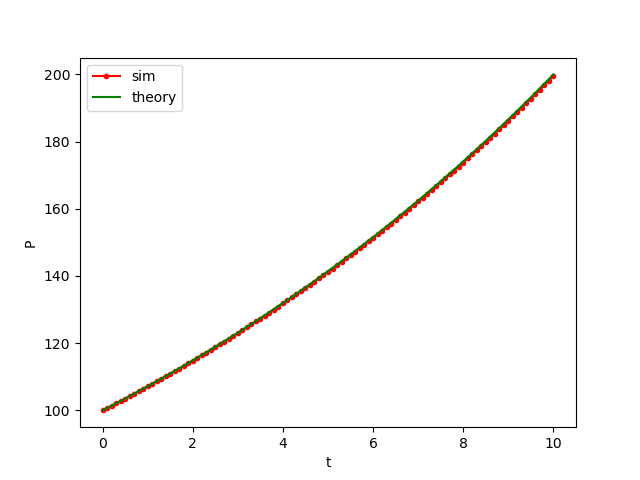
\includegraphics[width=0.8\textwidth]{figs/fig.png} % Ensure the image exists
\end{figure}
\end{frame}

\begin{frame}[fragile, allowframebreaks]{C Code: Generate the points}
\lstset{
        language = C,
        basicstyle=\ttfamily\tiny,
        keywordstyle=\color{blue},
        stringstyle=\color{green},
        commentstyle=\color{gray},
        tabsize=4
    }
    \lstinputlisting{./codes/points.c}
\end{frame}

\begin{frame}[fragile, allowframebreaks]{Python: To plot the points}
\lstset{
        language = Python,
        basicstyle=\ttfamily\tiny,
        keywordstyle=\color{blue},
        stringstyle=\color{green},
        commentstyle=\color{gray},
        tabsize=4
    }
    \lstinputlisting{./codes/plot.py}
\end{frame}


\end{document}
e
